\documentclass[conference,compsoc]{IEEEtran}
\usepackage[nocompress]{cite}
\usepackage[pdftex]{graphicx}
\usepackage[utf8]{inputenc}
\usepackage{amsmath}
\usepackage{amssymb}
\usepackage{amsthm}
\interdisplaylinepenalty=2500

\usepackage{algorithm}
\usepackage{algpseudocode}
\usepackage{url}
\usepackage{bm}
\usepackage{bbm}
\usepackage{multirow}
% \usepackage{pdflscape}
\usepackage[caption=false,font=footnotesize,labelfont=sf,textfont=sf]{subfig}

\title{Extended Appendix}

\begin{document}

\section{Further Performance Results}

In this section, we present the results from experiments showing the performance of 5 federated learning algorithms learning the CIFAR-10 task using the CNN1 model. We evaluated with a 10 client system with varying number of local client epochs and degree of data heterogeneity with the $\alpha$ parameterized LDA algorithm. This is to compare how our algorithm performed under differing settings. We found that while our algorithm is the best performing in a single epoch and in heterogeneous settings, it is outperformed by the more standard federated optimization algorithms. However, for the 3 to 10 epoch settings we are able to outperform the others with our algorithm by using a modified form of the FedAdam optimizer at the server side. This algorithm is applicable to ours ``out-of-the-box'' in settings where the aggregated global gradient is available to the server, and we found that it is better performing when the desired $\beta_1, \beta_2$ parameters were raised to the power of the number of local epochs clients performed.

\noindent Our algorithm combined with the modified FedAdam is not a catch-all, as for 1 or 2 epoch training there is too much influence from the moments. That is, past gradient estimations influence the current updates too much from overuse, derailing the learning process, while for 3-10 epochs there are sufficient gaps in moment application that past gradients are not misdirecting convergence.

\begin{table}[ht]
\centering
\caption{Performance of FedAVG}
    \centering
    \begin{tabular}{lll}
    \hline
    \textbf{$\alpha$} & \textbf{Epochs} & \textbf{Final accuracy $\uparrow$} \\
    \hline
    \multirow{10}{*}{0.1} & 1 & 70.363\% (0.892\%) \\
    & 2 & 67.979\% (1.904\%) \\
    & 3 & 66.623\% (0.787\%) \\
    & 4 & 64.704\% (1.857\%) \\
    & 5 & 62.874\% (1.552\%) \\
    & 10 & 60.727\% (2.411\%) \\
    & 15 & 59.605\% (3.666\%) \\
    & 20 & 58.771\% (3.063\%) \\
    & 25 & 58.864\% (2.390\%) \\
    & 30 & 58.106\% (2.804\%) \\
    \hline
    \multirow{10}{*}{0.5} & 1 & 69.635\% (4.393\%) \\
    & 2 & 71.558\% (1.138\%) \\
    & 3 & 71.261\% (0.708\%) \\
    & 4 & 70.777\% (1.576\%) \\
    & 5 & 70.753\% (1.039\%) \\
    & 10 & 70.085\% (1.078\%) \\
    & 15 & 69.868\% (1.104\%) \\
    & 20 & 69.201\% (0.957\%) \\
    & 25 & 69.488\% (1.120\%) \\
    & 30 & 69.020\% (1.220\%) \\
    \hline
    \multirow{10}{*}{1.0} & 1 & 72.910\% (0.516\%) \\
    & 2 & 72.703\% (0.586\%) \\
    & 3 & 72.403\% (0.308\%) \\
    & 4 & 71.932\% (0.324\%) \\
    & 5 & 72.439\% (0.362\%) \\
    & 10 & 72.085\% (0.451\%) \\
    & 15 & 72.202\% (0.739\%) \\
    & 20 & 71.548\% (0.767\%) \\
    & 25 & 71.548\% (0.675\%) \\
    & 30 & 71.731\% (0.507\%) \\
    \hline
    \multirow{10}{*}{10.0} & 1 & 73.034\% (1.016\%) \\
    & 2 & 73.381\% (0.405\%) \\
    & 3 & 73.007\% (0.267\%) \\
    & 4 & 73.271\% (0.507\%) \\
    & 5 & 73.074\% (0.986\%) \\
    & 10 & 73.180\% (0.417\%) \\
    & 15 & 72.897\% (0.401\%) \\
    & 20 & 73.067\% (0.173\%) \\
    & 25 & 72.680\% (0.485\%) \\
    & 30 & 72.726\% (0.253\%) \\
    \hline
    \end{tabular}
\end{table}

\begin{table}[ht]
\centering
\caption{Performance of FedAVG with Adam}
    \centering
    \begin{tabular}{lll}
    \hline
    $\alpha$ & \textbf{Epochs} & \textbf{Final accuracy $\uparrow$} \\
    \hline
    \multirow{10}{*}{0.1} & 1 & 29.016\% (3.256\%) \\
    & 2 & 51.058\% (6.337\%) \\
    & 3 & 56.657\% (5.801\%) \\
    & 4 & 56.317\% (4.618\%) \\
    & 5 & 57.345\% (4.786\%) \\
    & 10 & 56.370\% (5.781\%) \\
    & 15 & 56.147\% (5.254\%) \\
    & 20 & 52.350\% (8.666\%) \\
    & 25 & 52.891\% (7.930\%) \\
    & 30 & 53.539\% (3.266\%) \\
    \hline
    \multirow{10}{*}{0.5} & 1 & 60.784\% (8.650\%) \\
    & 2 & 71.775\% (1.063\%) \\
    & 3 & 72.346\% (1.499\%) \\
    & 4 & 72.433\% (1.533\%) \\
    & 5 & 72.092\% (1.704\%) \\
    & 10 & 71.631\% (2.106\%) \\
    & 15 & 71.638\% (1.388\%) \\
    & 20 & 71.782\% (1.493\%) \\
    & 25 & 71.805\% (1.280\%) \\
    & 30 & 71.534\% (1.579\%) \\
    \hline
    \multirow{10}{*}{1.0} & 1 & 69.601\% (3.237\%) \\
    & 2 & 73.875\% (1.343\%) \\
    & 3 & 74.376\% (0.998\%) \\
    & 4 & 74.189\% (0.637\%) \\
    & 5 & 74.215\% (0.582\%) \\
    & 10 & 74.349\% (0.808\%) \\
    & 15 & 74.269\% (0.486\%) \\
    & 20 & 73.985\% (0.320\%) \\
    & 25 & 74.015\% (0.559\%) \\
    & 30 & 74.493\% (0.775\%) \\
    \hline
    \multirow{10}{*}{10.0} & 1 & 75.501\% (0.381\%) \\
    & 2 & 75.317\% (0.658\%) \\
    & 3 & 75.187\% (0.119\%) \\
    & 4 & 75.765\% (0.583\%) \\
    & 5 & 75.634\% (0.399\%) \\
    & 10 & 75.758\% (0.488\%) \\
    & 15 & 75.771\% (0.364\%) \\
    & 20 & 76.008\% (0.993\%) \\
    & 25 & 76.075\% (0.579\%) \\
    & 30 & 75.931\% (1.102\%) \\
    \hline
    \end{tabular}
\end{table}

\begin{table}[ht]
\centering
\caption{Performance of FedAdam}
\begin{tabular}{lll}
\hline
$\alpha$ & \textbf{Epochs} & \textbf{Final accuracy $\uparrow$} \\
\hline
\multirow{10}{*}{0.1} & 1 & 54.050\% (3.466\%) \\
& 2 & 9.996\% (0.017\%) \\
& 3 & 40.792\% (26.681\%) \\
& 4 & 54.400\% (1.150\%) \\
& 5 & 58.270\% (0.511\%) \\
& 10 & 51.112\% (4.641\%) \\
& 15 & 54.858\% (3.477\%) \\
& 20 & 54.470\% (3.750\%) \\
& 25 & 54.734\% (3.307\%) \\
& 30 & 50.942\% (4.746\%) \\
\hline
\multirow{10}{*}{0.5} & 1 & 27.574\% (30.455\%) \\
& 2 & 26.659\% (28.853\%) \\
& 3 & 43.480\% (29.482\%) \\
& 4 & 63.211\% (0.972\%) \\
& 5 & 62.440\% (2.560\%) \\
& 10 & 62.951\% (0.852\%) \\
& 15 & 62.907\% (2.274\%) \\
& 20 & 66.042\% (1.441\%) \\
& 25 & 64.370\% (1.989\%) \\
& 30 & 64.173\% (0.824\%) \\
\hline
\multirow{10}{*}{1.0} & 1 & 24.820\% (25.667\%) \\
& 2 & 25.494\% (26.835\%) \\
& 3 & 61.705\% (2.327\%) \\
& 4 & 63.438\% (1.275\%) \\
& 5 & 62.043\% (2.541\%) \\
& 10 & 65.615\% (1.649\%) \\
& 15 & 66.173\% (1.564\%) \\
& 20 & 65.398\% (3.004\%) \\
& 25 & 67.748\% (2.031\%) \\
& 30 & 66.246\% (3.975\%) \\
\hline
\multirow{10}{*}{10.0} & 1 & 38.866\% (25.223\%) \\
& 2 & 10.013\% (0.006\%) \\
& 3 & 64.026\% (0.614\%) \\
& 4 & 64.373\% (2.145\%) \\
& 5 & 66.436\% (1.809\%) \\
& 10 & 68.079\% (1.182\%) \\
& 15 & 68.950\% (0.874\%) \\
& 20 & 68.954\% (2.209\%) \\
& 25 & 70.409\% (0.794\%) \\
& 30 & 70.376\% (0.787\%) \\
\hline
\end{tabular}
\end{table} 


\begin{table}[ht]
\centering
\caption{Performance of our proposed algorithm}
    \centering
    \begin{tabular}{lll}
    \hline
    $\alpha$ & \textbf{Epochs} & \textbf{Final accuracy $\uparrow$} \\
    \hline
    \multirow{10}{*}{0.1} & 1 & 70.880\% (0.236\%) \\
    & 2 & 68.069\% (0.794\%) \\
    & 3 & 63.478\% (1.673\%) \\
    & 4 & 59.145\% (2.144\%) \\
    & 5 & 55.946\% (2.558\%) \\
    & 10 & 43.717\% (2.604\%) \\
    & 15 & 32.799\% (5.444\%) \\
    & 20 & 23.170\% (6.714\%) \\
    & 25 & 19.224\% (4.748\%) \\
    & 30 & 22.923\% (0.981\%) \\
    \hline
    \multirow{10}{*}{0.5} & 1 & 74.192\% (0.502\%) \\
    & 2 & 73.264\% (1.212\%) \\
    & 3 & 70.800\% (1.619\%) \\
    & 4 & 68.129\% (1.210\%) \\
    & 5 & 65.658\% (1.038\%) \\
    & 10 & 50.027\% (0.866\%) \\
    & 15 & 34.635\% (3.083\%) \\
    & 20 & 24.947\% (5.759\%) \\
    & 25 & 22.589\% (4.772\%) \\
    & 30 & 24.793\% (7.588\%) \\
    \hline
    \multirow{10}{*}{1.0} & 1 & 75.307\% (0.360\%) \\
    & 2 & 74.429\% (0.135\%) \\
    & 3 & 72.035\% (0.539\%) \\
    & 4 & 70.336\% (0.399\%) \\
    & 5 & 67.805\% (0.986\%) \\
    & 10 & 50.177\% (0.417\%) \\
    & 15 & 41.069\% (2.850\%) \\
    & 20 & 21.999\% (3.115\%) \\
    & 25 & 29.704\% (6.101\%) \\
    & 30 & 22.196\% (7.389\%) \\
    \hline
    \multirow{10}{*}{10.0} & 1 & 75.972\% (0.536\%) \\
    & 2 & 74.866\% (0.273\%) \\
    & 3 & 73.054\% (0.214\%) \\
    & 4 & 71.334\% (0.777\%) \\
    & 5 & 69.294\% (0.807\%) \\
    & 10 & 49.593\% (1.311\%) \\
    & 15 & 41.196\% (0.994\%) \\
    & 20 & 32.278\% (2.564\%) \\
    & 25 & 21.645\% (3.658\%) \\
    & 30 & 24.442\% (11.040\%) \\
    \hline
    \end{tabular}
\end{table}

\begin{table}[ht]
\centering
\caption{Performance of our proposed algorithm with FedAdam aggregation}
    \centering
    \begin{tabular}{lll}
    \hline
    $\alpha$ & \textbf{Epochs} & \textbf{Final accuracy $\uparrow$} \\
    \hline
    \multirow{10}{*}{0.1} & 1 & 50.200\% (2.480\%) \\
    & 2 & 58.327\% (4.164\%) \\
    & 3 & 63.729\% (3.235\%) \\
    & 4 & 70.887\% (0.729\%) \\
    & 5 & 69.408\% (1.827\%) \\
    & 10 & 67.752\% (1.421\%) \\
    & 15 & 60.263\% (0.678\%) \\
    & 20 & 50.651\% (6.358\%) \\
    & 25 & 47.700\% (2.178\%) \\
    & 30 & 33.420\% (3.145\%) \\
    \hline
    \multirow{10}{*}{0.5} & 1 & 49.890\% (4.009\%) \\
    & 2 & 64.830\% (1.455\%) \\
    & 3 & 72.419\% (1.663\%) \\
    & 4 & 73.725\% (1.862\%) \\
    & 5 & 74.554\% (0.992\%) \\
    & 10 & 72.010\% (0.935\%) \\
    & 15 & 58.691\% (5.379\%) \\
    & 20 & 58.420\% (2.796\%) \\
    & 25 & 48.655\% (7.004\%) \\
    & 30 & 29.760\% (8.406\%) \\
    \hline
    \multirow{10}{*}{1.0} & 1 & 34.265\% (21.087\%) \\
    & 2 & 66.373\% (1.567\%) \\
    & 3 & 72.786\% (0.800\%) \\
    & 4 & 75.397\% (0.286\%) \\
    & 5 & 75.270\% (0.256\%) \\
    & 10 & 74.245\% (0.291\%) \\
    & 15 & 59.332\% (5.201\%) \\
    & 20 & 53.105\% (10.382\%) \\
    & 25 & 45.600\% (2.616\%) \\
    & 30 & 28.559\% (2.342\%) \\
    \hline
    \multirow{10}{*}{10.0} & 1 & 34.943\% (21.605\%) \\
    & 2 & 68.884\% (0.723\%) \\
    & 3 & 74.382\% (0.316\%) \\
    & 4 & 75.848\% (0.336\%) \\
    & 5 & 75.671\% (1.092\%) \\
    & 10 & 73.698\% (1.535\%) \\
    & 15 & 58.086\% (5.665\%) \\
    & 20 & 48.865\% (6.932\%) \\
    & 25 & 41.510\% (5.488\%) \\
    & 30 & 33.407\% (5.987\%) \\
    \hline
    \end{tabular}
\end{table}


\section{Datasets}

In this section we provide brief descriptions of the datasets that we have used in our experiments and the pre-processing that we have applied.

\subsection{Fashion-MNIST}

Fashion-MNIST \cite{xiao2017fashion} was created as a drop-in replacement for the immensely popular MNIST dataset \cite{lecun1998gradient}, and has equivalent structure while providing a more complex learning task. The dataset is composed of 70 000 grayscale images with $28 \times 28$ pixels, where each image belongs to one of ten classes, in this case denoting the item of clothing the image is made of (e.g. trouser and dress). 60 000 of these images are in the training dataset, and the other 10 000 in the testing dataset.

\noindent For pre-processing, we first scaled the images from their byte-per-pixel encoding into a floating point in the range $[0, 1]$ for each pixel by dividing their value by $255$. We then converted each resulting sample into a 3D array with shape $28 \times 28 \times 1$.

\subsection{CIFAR-10}

CIFAR-10 \cite{krizhevsky2009learning} is an object classification dataset composed of 60 000 RGB color images with $32 \times 32$ pixels, with 50 000 samples in the training dataset and 10 000 in the testing dataset. It was created as a subset of the tiny images dataset\footnote{The tiny images dataset was formally withdrawn as specified at \url{https://groups.csail.mit.edu/vision/TinyImages/}}, where reliable class labels are ensured for improved learning quality. The dataset has 10 classes, where each sample is labeled with the one it is an image of (e.g. cat, ship, airplane, etc.).

\noindent To pre-process this dataset, we first standardize the data from the byte-per-pixel-channel format to floating points in the range $[0, 1]$ for each pixel-channel by an element-wise division by $255$. We then cast each sample into a 3D array with shape $32 \times 32 \times 3$.

\subsection{SVHN}

SVHN \cite{netzer2011svhn} is a digit recognition dataset similar to the MNIST dataset \cite{lecun1998gradient}, while providing a significantly harder learning task by using images obtained from real-world house numbers with various natural scenes. We use the cropped digits format of the dataset, which is composed of 99289 RGB color images with $32 \times 32$ pixels, where training dataset contains 73257 samples and the testing dataset contains 26032 samples. Each sample is labeled with one of 10 classes stating which digit is contained in the respective image.


\section{Projected Gradient Descent}

Unless stated otherwise, we have used the projected gradient descent algorithm \cite{goodfellow2014explaining} as an adversarial training step each epoch of training in each experiment. For this algorithm, we set the learning rate, $\eta_{pgd}$, to 1\% of the primary task learning rate, the maximum amount of perturbation, $\epsilon$, to $0.3$, and the number of steps, $S$, to 1. The specific algorithm we have used is demonstrated in Algorithm \ref{alg:pgd}.


\begin{algorithm}[H]
\caption{Projected Gradient Descent}
\label{alg:pgd}
\begin{algorithmic}[1]
    \Function{PGD}{objective function evaluated with the current model $F_{\bm{\theta}}$, maximum amount of perturbation $\epsilon$, learning rate $\eta_{pgd}$, number of steps $S$, minibatch samples $\bm{X}$, minibatch labels $\bm{y}$}
        \State $\bm{X}_0 \gets \bm{X}$
        \For{\textbf{each} step $s \in [S]$}
            \State $\bm{g}_s \gets \nabla_{\bm{X}} F_{\bm{\theta}}(\bm{X}, \bm{y})$
            \State $\bm{X}_s \gets \bm{X} + \eta_{pgd} \text{sign}(\bm{g}_s)$
            \State $\bm{X}_s \gets \text{clip}(\bm{X}_s, \bm{X} - \epsilon, \bm{X} + \epsilon$)
        \EndFor
        \State \Return $\bm{X}_S$
    \EndFunction
\end{algorithmic}
\end{algorithm}


\section{Samples of Backdoor Data}\label{sec:triggers}

\begin{figure}[ht]
    \centering
    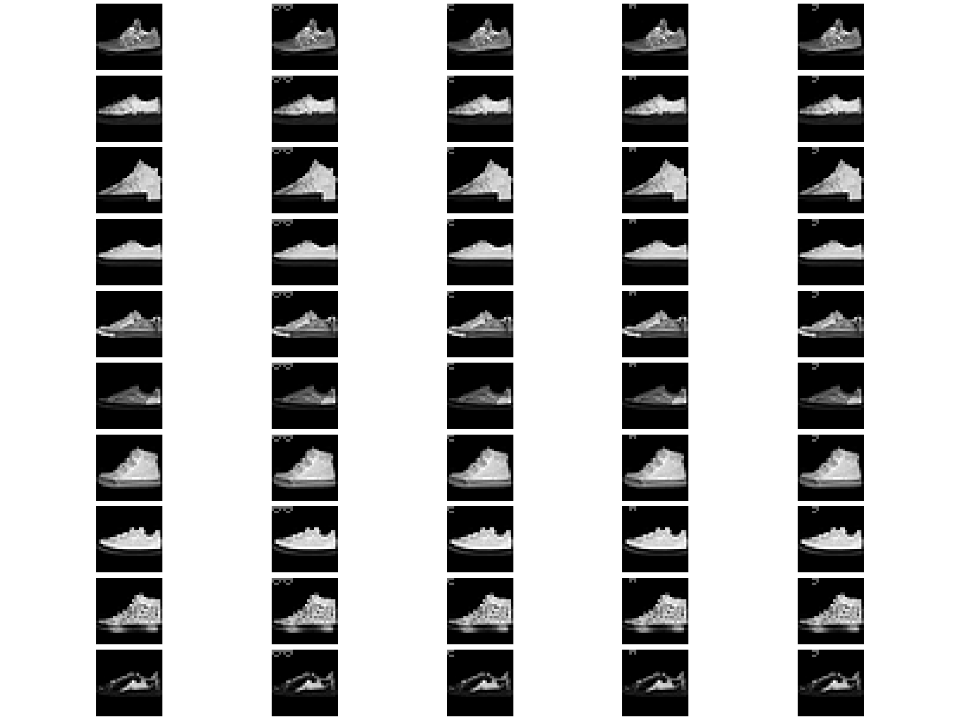
\includegraphics[width=\columnwidth]{images/backdoor/triggers.pdf}
    \caption{Samples of the backdoor data. First column shows the ground truth, second column shows the full pixel pattern trigger, and the last three columns show each of the thirds of the trigger used in the distributed attack.}
    \label{fig:triggers}
\end{figure}



\section{Classifier Metric}

For our classifier metric we trained the CNN shown in Table~\ref{table:cm_cnn} of FMNIST, DenseNet-BC-190 for CIFAR-10, and DenseNet121 for SVHN. Each model was trained for 3000 steps with a minibatch size of 512, using the the yogi~\cite{zaheer2018yogi} optimizer with a learning rate $10^{-3}$, $\beta_1 = 0.9$, $\beta_2 = 0.999$, and $\varepsilon = 0.001$.

\begin{table}[H]
\centering
\caption{CNN used for the FMNIST classifier metric}
\label{table:cm_cnn}
\begin{tabular}{ll}
\hline
\textbf{Layer Type} & \textbf{Hyperparameters} \\
\hline
Convolutional & $32$ filters, $3 \times 3$ kernel, $2 \times 2$ strides \\
Batch Normalization & Depth axis, $\varepsilon = 1.001 \times 10^{-5}$ \\
ReLU & \\
Convolutional & $32$ filters, $3 \times 3$ kernel, $2 \times 2$ strides \\
Batch Normalization & Depth axis, $\varepsilon = 1.001 \times 10^{-5}$ \\
ReLU & \\
Max Pooling & $3 \times 3$ kernel, $2 \times 2$ strides \\
Convolutional & $64$ filters, $3 \times 3$ kernel, $2 \times 2$ strides \\
Batch Normalization & Depth axis, $\varepsilon = 1.001 \times 10^{-5}$ \\
ReLU & \\
Convolutional & $64$ filters, $3 \times 3$ kernel, $2 \times 2$ strides \\
Batch Normalization & Depth axis, $\varepsilon = 1.001 \times 10^{-5}$ \\
ReLU & \\
Global Average Pooling & \\
Dense & $\# Classes$ neurons \\
Softmax & \\
\hline
\end{tabular}
\end{table}

\section{Full Mitigation Results}\label{sec:full_mitigation_results}

\begin{table}[H]
\centering
\caption{Base algorithm against the continuous attack. Certified accuracy and certified ASR were always 0 - they never recover from the attack}
\begin{tabular}{lllll}
\hline
\textbf{Dataset} & \textbf{Model} & \textbf{Final ACC} $\uparrow$ & \textbf{First ASR} $\downarrow$ & \textbf{Final ASR} $\downarrow$ \\
\hline
\multirow{3}{*}{FMNIST} & LeNet & 88.258\% (0.263\%) & 0.000\% (0.000\%) & 100.000\% (0.000\%) \\
& CNN1 & 92.004\% (0.259\%) & 27.755\% (35.594\%) & 100.000\% (0.000\%) \\
& CNN2 & 93.059\% (0.444\%) & 89.483\% (16.670\%) & 100.000\% (0.000\%) \\
\hline
\multirow{3}{*}{CIFAR-10} & LeNet & 49.346\% (0.067\%) & 9.913\% (6.784\%) & 38.810\% (1.666\%) \\
& CNN1 & 70.052\% (1.407\%) & 20.531\% (8.616\%) & 45.867\% (12.873\%) \\
& CNN2 & 68.977\% (0.629\%) & 53.427\% (38.712\%) & 42.305\% (3.018\%) \\
\hline
\multirow{3}{*}{SVHN} & LeNet & 68.477\% (1.009\%) & 6.498\% (1.207\%) & 58.879\% (7.849\%) \\
& CNN1 & 85.041\% (0.904\%) & 40.890\% (18.386\%) & 74.173\% (9.793\%) \\
& CNN2 & 84.803\% (2.291\%) & 99.818\% (0.273\%) & 76.091\% (3.911\%) \\
\hline
\end{tabular}
\end{table}

\newpage

\begin{landscape}

\begin{table}[H]
\centering
\caption{Base algorithm against the one-shot attack}
\begin{tabular}{llllllll}
\hline
\textbf{Dataset} & \textbf{Model} & \textbf{Certified ACC} $\uparrow$ & \textbf{Certified ASR} $\downarrow$ & \textbf{Final ACC} $\uparrow$ & \textbf{First ASR} $\downarrow$ & \textbf{Final ASR} $\downarrow$ & \textbf{Recovery rounds} $\downarrow$ \\
\hline
\multirow{3}{*}{FMNIST} & LeNet & 87.193\% (0.170\%) & 0.000\% (0.000\%) & 88.318\% (0.194\%) & 8.837\% (7.460\%) & 0.000\% (0.000\%) & 0.667 (0.577) \\
& CNN1 & 88.261\% (1.846\%) & 0.000\% (0.000\%) & 90.859\% (1.195\%) & 100.000\% (0.000\%) & 0.000\% (0.000\%) & 0.667 (0.577) \\
& CNN2 & 0.000\% (0.000\%) & 0.000\% (0.000\%) & 93.296\% (0.061\%) & 99.059\% (1.630\%) & 0.000\% (0.000\%) & 0.667 (1.155) \\
\hline
\multirow{3}{*}{CIFAR-10} & LeNet & 48.274\% (1.387\%) & 11.761\% (5.296\%) & 50.945\% (0.406\%) & 70.867\% (50.373\%) & 7.728\% (3.452\%) & 2.667 (1.155) \\
& CNN1 & 67.318\% (2.076\%) & 1.949\% (1.030\%) & 73.444\% (0.403\%) & 91.700\% (14.376\%) & 4.167\% (0.254\%) & 1.000 (0.000) \\
& CNN2 & 0.000\% (0.000\%) & 0.000\% (0.000\%) & 72.029\% (0.223\%) & 100.000\% (0.000\%) & 3.797\% (0.455\%) & 1.000 (0.000) \\
\hline
\multirow{3}{*}{SVHN} & LeNet & 69.350\% (2.274\%) & 6.663\% (5.723\%) & 72.052\% (0.278\%) & 68.535\% (51.844\%) & 3.042\% (0.592\%) & 1.667 (0.577) \\
& CNN1 & 80.841\% (2.984\%) & 4.431\% (3.971\%) & 87.080\% (3.754\%) & 100.000\% (0.000\%) & 1.025\% (0.348\%) & 0.333 (0.577) \\
& CNN2 & 0.000\% (0.000\%) & 0.000\% (0.000\%) & 89.377\% (0.347\%) & 67.262\% (55.634\%) & 1.290\% (0.216\%) & 2.333 (2.309) \\
\hline
\end{tabular}
\end{table}

\begin{table}[H]
\centering
\caption{Noising and clipping method against the continuous attack}
\begin{tabular}{llllllll}
\hline
\textbf{Dataset} & \textbf{Model} & \textbf{Certified ACC} $\uparrow$ & \textbf{Certified ASR} $\downarrow$ & \textbf{Final ACC} $\uparrow$ & \textbf{First ASR} $\downarrow$ & \textbf{Final ASR} $\downarrow$ & \textbf{Recovery rounds} $\downarrow$ \\
\hline
\multirow{3}{*}{FMNIST} & LeNet & 0.000\% (0.000\%) & 0.000\% (0.000\%) & 65.762\% (1.593\%) & 0.000\% (0.000\%) & 51.109\% (16.122\%) & 0.000 (0.000) \\
& CNN1 & 0.000\% (0.000\%) & 0.000\% (0.000\%) & 71.938\% (0.562\%) & 0.000\% (0.000\%) & 62.366\% (5.918\%) & 0.000 (0.000) \\
& CNN2 & 0.000\% (0.000\%) & 0.000\% (0.000\%) & 87.987\% (0.215\%) & 0.000\% (0.000\%) & 100.000\% (0.000\%) & 0.000 (0.000) \\
\hline
\multirow{3}{*}{CIFAR-10} & LeNet & 0.000\% (0.000\%) & 0.000\% (0.000\%) & 33.771\% (0.560\%) & 6.048\% (2.024\%) & 42.137\% (2.358\%) & 0.000 (0.000) \\
& CNN1 & 0.000\% (0.000\%) & 0.000\% (0.000\%) & 39.590\% (0.878\%) & 7.897\% (3.001\%) & 46.875\% (5.288\%) & 0.000 (0.000) \\
& CNN2 & 0.000\% (0.000\%) & 0.000\% (0.000\%) & 51.739\% (0.872\%) & 5.242\% (1.659\%) & 35.148\% (3.894\%) & 0.000 (0.000) \\
\hline
\multirow{3}{*}{SVHN} & LeNet & 0.000\% (0.000\%) & 0.000\% (0.000\%) & 29.191\% (1.036\%) & 0.942\% (0.347\%) & 75.182\% (4.032\%) & 0.000 (0.000) \\
& CNN1 & 0.000\% (0.000\%) & 0.000\% (0.000\%) & 37.582\% (0.890\%) & 2.050\% (2.185\%) & 64.038\% (11.371\%) & 0.000 (0.000) \\
& CNN2 & 0.000\% (0.000\%) & 0.000\% (0.000\%) & 70.434\% (2.440\%) & 2.364\% (0.949\%) & 46.032\% (5.337\%) & 0.000 (0.000) \\
\hline
\end{tabular}
\end{table}

\begin{table}[H]
\centering
\caption{Noising and clipping method against the one-shot attack}
\begin{tabular}{llllllll}
\hline
\textbf{Dataset} & \textbf{Model} & \textbf{Certified ACC} $\uparrow$ & \textbf{Certified ASR} $\downarrow$ & \textbf{Final ACC} $\uparrow$ & \textbf{First ASR} $\downarrow$ & \textbf{Final ASR} $\downarrow$ & \textbf{Recovery rounds} $\downarrow$ \\
\hline
\multirow{3}{*}{FMNIST} & LeNet & 70.940\% (0.621\%) & 0.000\% (0.000\%) & 71.391\% (0.880\%) & 0.000\% (0.000\%) & 0.000\% (0.000\%) & 0.000 (0.000) \\
& CNN1 & 71.441\% (5.340\%) & 0.000\% (0.000\%) & 78.536\% (0.759\%) & 0.000\% (0.000\%) & 0.000\% (0.000\%) & 0.000 (0.000) \\
& CNN2 & 0.000\% (0.000\%) & 0.000\% (0.000\%) & 88.502\% (0.121\%) & 0.000\% (0.000\%) & 0.000\% (0.000\%) & 0.000 (0.000) \\
\hline
\multirow{3}{*}{CIFAR-10} & LeNet & 34.145\% (0.643\%) & 13.710\% (6.631\%) & 37.053\% (0.143\%) & 6.216\% (2.017\%) & 5.880\% (1.664\%) & 999.000 (0.000) \\
& CNN1 & 34.178\% (7.198\%) & 10.517\% (15.102\%) & 42.421\% (0.772\%) & 8.367\% (3.262\%) & 6.720\% (2.433\%) & 999.000 (0.000) \\
& CNN2 & 0.000\% (0.000\%) & 0.000\% (0.000\%) & 54.497\% (0.608\%) & 5.544\% (1.067\%) & 5.612\% (0.915\%) & 999.000 (0.000) \\
\hline
\multirow{3}{*}{SVHN} & LeNet & 28.823\% (4.557\%) & 2.960\% (3.549\%) & 36.075\% (0.664\%) & 0.992\% (0.455\%) & 1.438\% (0.473\%) & 333.000 (576.773) \\
& CNN1 & 39.023\% (4.453\%) & 26.571\% (36.841\%) & 42.968\% (0.297\%) & 2.133\% (2.181\%) & 3.869\% (2.198\%) & 342.000 (569.139) \\
& CNN2 & 0.000\% (0.000\%) & 0.000\% (0.000\%) & 75.269\% (1.912\%) & 2.331\% (0.603\%) & 2.116\% (0.862\%) & 634.667 (504.377) \\
\hline
\end{tabular}
\end{table}

\begin{table}[H]
\centering
\caption{Algorithm with PGD hardening method against the continuous attack - does not recover}
\begin{tabular}{llllllll}
\hline
\textbf{Dataset} & \textbf{Model} & $\varepsilon$ & \textbf{Certified ACC} $\uparrow$ & \textbf{Certified ASR} $\downarrow$ & \textbf{Final ACC} $\uparrow$ & \textbf{First ASR} $\downarrow$ & \textbf{Final ASR} $\downarrow$ \\
\hline
\multirow{12}{*}{FMNIST} & \multirow{4}{*}{LeNet} & 0.010 & 86.952\% (0.122\%) & 99.966\% (0.058\%) & 88.268\% (0.333\%) & 0.000\% (0.000\%) & 100.000\% (0.000\%) \\
& & 0.100 & 0.000\% (0.000\%) & 0.000\% (0.000\%) & 88.268\% (0.333\%) & 0.000\% (0.000\%) & 100.000\% (0.000\%) \\
& & 0.500 & 0.000\% (0.000\%) & 0.000\% (0.000\%) & 88.268\% (0.333\%) & 0.000\% (0.000\%) & 100.000\% (0.000\%) \\
& & 1.000 & 0.000\% (0.000\%) & 0.000\% (0.000\%) & 88.268\% (0.333\%) & 0.000\% (0.000\%) & 100.000\% (0.000\%) \\
\cline{2-8}
& \multirow{4}{*}{CNN1} & 0.010 & 85.667\% (3.857\%) & 99.933\% (0.116\%) & 91.977\% (0.148\%) & 33.098\% (36.378\%) & 100.000\% (0.000\%) \\
& & 0.100 & 0.000\% (0.000\%) & 0.000\% (0.000\%) & 92.037\% (0.208\%) & 25.202\% (34.224\%) & 100.000\% (0.000\%) \\
& & 0.500 & 0.000\% (0.000\%) & 0.000\% (0.000\%) & 92.081\% (0.180\%) & 28.931\% (42.717\%) & 100.000\% (0.000\%) \\
& & 1.000 & 0.000\% (0.000\%) & 0.000\% (0.000\%) & 91.877\% (0.244\%) & 28.427\% (37.088\%) & 100.000\% (0.000\%) \\
\cline{2-8}
& \multirow{4}{*}{CNN2} & 0.010 & 86.325\% (4.403\%) & 100.000\% (0.000\%) & 93.166\% (0.187\%) & 66.599\% (57.677\%) & 100.000\% (0.000\%) \\
& & 0.100 & 0.000\% (0.000\%) & 0.000\% (0.000\%) & 92.925\% (0.507\%) & 66.532\% (57.619\%) & 100.000\% (0.000\%) \\
& & 0.500 & 0.000\% (0.000\%) & 0.000\% (0.000\%) & 92.969\% (0.290\%) & 100.000\% (0.000\%) & 100.000\% (0.000\%) \\
& & 1.000 & 0.000\% (0.000\%) & 0.000\% (0.000\%) & 93.106\% (0.165\%) & 0.437\% (0.382\%) & 100.000\% (0.000\%) \\
\hline
\multirow{12}{*}{CIFAR-10} & \multirow{4}{*}{LeNet} & 0.010 & 45.853\% (1.542\%) & 50.202\% (16.003\%) & 49.192\% (0.176\%) & 9.913\% (5.373\%) & 41.465\% (4.996\%) \\
& & 0.100 & 0.000\% (0.000\%) & 0.000\% (0.000\%) & 49.192\% (0.176\%) & 9.913\% (5.373\%) & 41.465\% (4.996\%) \\
& & 0.500 & 0.000\% (0.000\%) & 0.000\% (0.000\%) & 49.192\% (0.176\%) & 9.913\% (5.373\%) & 41.465\% (4.996\%) \\
& & 1.000 & 0.000\% (0.000\%) & 0.000\% (0.000\%) & 49.192\% (0.176\%) & 9.913\% (5.373\%) & 41.465\% (4.996\%) \\
\cline{2-8}
& \multirow{4}{*}{CNN1} & 0.010 & 62.934\% (2.992\%) & 45.934\% (13.165\%) & 69.922\% (0.951\%) & 20.800\% (8.583\%) & 45.901\% (10.177\%) \\
& & 0.100 & 0.000\% (0.000\%) & 0.000\% (0.000\%) & 69.925\% (1.825\%) & 20.464\% (8.155\%) & 48.421\% (18.999\%) \\
& & 0.500 & 0.000\% (0.000\%) & 0.000\% (0.000\%) & 70.059\% (1.176\%) & 19.825\% (7.913\%) & 45.934\% (13.358\%) \\
& & 1.000 & 0.000\% (0.000\%) & 0.000\% (0.000\%) & 70.192\% (2.120\%) & 19.422\% (7.716\%) & 46.035\% (22.821\%) \\
\cline{2-8}
& \multirow{4}{*}{CNN2} & 0.010 & 51.790\% (2.905\%) & 61.996\% (11.316\%) & 67.859\% (0.607\%) & 86.425\% (22.815\%) & 45.195\% (10.832\%) \\
& & 0.100 & 0.000\% (0.000\%) & 0.000\% (0.000\%) & 68.490\% (0.833\%) & 80.847\% (32.564\%) & 38.071\% (8.874\%) \\
& & 0.500 & 0.000\% (0.000\%) & 0.000\% (0.000\%) & 68.239\% (0.934\%) & 99.362\% (0.354\%) & 45.329\% (10.976\%) \\
& & 1.000 & 0.000\% (0.000\%) & 0.000\% (0.000\%) & 67.628\% (1.136\%) & 98.555\% (1.078\%) & 53.360\% (2.470\%) \\
\hline
\multirow{12}{*}{SVHN} & \multirow{4}{*}{LeNet} & 0.010 & 64.987\% (3.035\%) & 59.788\% (14.691\%) & 69.013\% (1.113\%) & 8.052\% (1.839\%) & 55.456\% (12.281\%) \\
& & 0.100 & 0.000\% (0.000\%) & 0.000\% (0.000\%) & 69.013\% (1.113\%) & 8.052\% (1.839\%) & 55.456\% (12.281\%) \\
& & 0.500 & 0.000\% (0.000\%) & 0.000\% (0.000\%) & 69.013\% (1.113\%) & 8.052\% (1.839\%) & 55.456\% (12.281\%) \\
& & 1.000 & 0.000\% (0.000\%) & 0.000\% (0.000\%) & 69.013\% (1.113\%) & 8.052\% (1.839\%) & 55.456\% (12.281\%) \\
\cline{2-8}
& \multirow{4}{*}{CNN1} & 0.010 & 82.126\% (2.684\%) & 50.579\% (16.139\%) & 84.991\% (0.622\%) & 43.981\% (14.236\%) & 72.652\% (9.192\%) \\
& & 0.100 & 0.000\% (0.000\%) & 0.000\% (0.000\%) & 84.954\% (0.348\%) & 46.594\% (14.442\%) & 72.603\% (5.186\%) \\
& & 0.500 & 0.000\% (0.000\%) & 0.000\% (0.000\%) & 85.126\% (0.728\%) & 46.577\% (15.862\%) & 71.247\% (8.944\%) \\
& & 1.000 & 0.000\% (0.000\%) & 0.000\% (0.000\%) & 84.871\% (0.306\%) & 45.536\% (11.075\%) & 74.074\% (5.215\%) \\
\cline{2-8}
& \multirow{4}{*}{CNN2} & 0.010 & 69.607\% (12.020\%) & 88.558\% (3.614\%) & 84.180\% (0.608\%) & 100.000\% (0.000\%) & 72.983\% (11.013\%) \\
& & 0.100 & 0.000\% (0.000\%) & 0.000\% (0.000\%) & 86.219\% (0.934\%) & 87.070\% (22.266\%) & 67.593\% (13.141\%) \\
& & 0.500 & 0.000\% (0.000\%) & 0.000\% (0.000\%) & 83.469\% (0.934\%) & 100.000\% (0.000\%) & 73.082\% (4.581\%) \\
& & 1.000 & 0.000\% (0.000\%) & 0.000\% (0.000\%) & 85.898\% (0.369\%) & 67.063\% (54.195\%) & 70.023\% (8.548\%) \\
\hline
\end{tabular}
\end{table}


\begin{table}[H]
\centering
\caption{Algorithm with PGD against the one-shot attack}
\begin{tabular}{lllllllll}
\hline
\textbf{Dataset} & \textbf{Model} & $\varepsilon$ & \textbf{Certified ACC} $\uparrow$ & \textbf{Certified ASR} $\downarrow$ & \textbf{Final ACC} $\uparrow$ & \textbf{First ASR} $\downarrow$ & \textbf{Final ASR} $\downarrow$ & \textbf{Recovery} $\downarrow$ \\
\hline
\multirow{12}{*}{FMNIST} & \multirow{4}{*}{LeNet} & 0.010 & 87.216\% (0.115\%) & 0.000\% (0.000\%) & 88.425\% (0.182\%) & 8.199\% (7.046\%) & 0.000\% (0.000\%) & 0.667 (0.577) \\
& & 0.100 & 87.216\% (0.115\%) & 0.000\% (0.000\%) & 88.425\% (0.182\%) & 8.199\% (7.046\%) & 0.000\% (0.000\%) & 0.667 (0.577) \\
& & 0.500 & 0.000\% (0.000\%) & 0.000\% (0.000\%) & 88.425\% (0.182\%) & 8.199\% (7.046\%) & 0.000\% (0.000\%) & 0.667 (0.577) \\
& & 1.000 & 0.000\% (0.000\%) & 0.000\% (0.000\%) & 88.425\% (0.182\%) & 8.199\% (7.046\%) & 0.000\% (0.000\%) & 0.667 (0.577) \\
\cline{2-9}
& \multirow{4}{*}{CNN1} & 0.010 & 87.520\% (2.097\%) & 0.000\% (0.000\%) & 90.612\% (1.404\%) & 100.000\% (0.000\%) & 0.000\% (0.000\%) & 1.000 (0.000) \\
& & 0.100 & 88.408\% (1.165\%) & 0.000\% (0.000\%) & 90.809\% (1.144\%) & 100.000\% (0.000\%) & 0.000\% (0.000\%) & 1.000 (0.000) \\
& & 0.500 & 0.000\% (0.000\%) & 0.000\% (0.000\%) & 91.149\% (0.745\%) & 100.000\% (0.000\%) & 0.000\% (0.000\%) & 1.000 (0.000) \\
& & 1.000 & 0.000\% (0.000\%) & 0.000\% (0.000\%) & 90.939\% (1.128\%) & 100.000\% (0.000\%) & 0.000\% (0.000\%) & 1.000 (0.000) \\
\cline{2-9}
& \multirow{4}{*}{CNN2} & 0.010 & 88.061\% (3.641\%) & 1.344\% (2.072\%) & 93.199\% (0.226\%) & 99.866\% (0.233\%) & 0.302\% (0.363\%) & 0.667 (1.155) \\
& & 0.100 & 86.285\% (2.890\%) & 0.302\% (0.175\%) & 93.263\% (0.163\%) & 76.579\% (40.566\%) & 0.437\% (0.308\%) & 0.333 (0.577) \\
& & 0.500 & 0.000\% (0.000\%) & 0.000\% (0.000\%) & 93.269\% (0.050\%) & 100.000\% (0.000\%) & 0.941\% (0.616\%) & 0.333 (0.577) \\
& & 1.000 & 0.000\% (0.000\%) & 0.000\% (0.000\%) & 93.259\% (0.050\%) & 100.000\% (0.000\%) & 0.840\% (0.857\%) & 0.333 (0.577) \\
\hline
\multirow{12}{*}{CIFAR-10} & \multirow{4}{*}{LeNet} & 0.010 & 48.017\% (1.527\%) & 11.122\% (6.464\%) & 51.219\% (0.546\%) & 77.151\% (39.576\%) & 6.384\% (2.175\%) & 2.333 (0.577) \\
& & 0.100 & 48.017\% (1.527\%) & 11.122\% (6.464\%) & 51.219\% (0.546\%) & 77.151\% (39.576\%) & 6.384\% (2.175\%) & 2.333 (0.577) \\
& & 0.500 & 0.000\% (0.000\%) & 0.000\% (0.000\%) & 51.219\% (0.546\%) & 77.151\% (39.576\%) & 6.384\% (2.175\%) & 2.333 (0.577) \\
& & 1.000 & 0.000\% (0.000\%) & 0.000\% (0.000\%) & 51.219\% (0.546\%) & 77.151\% (39.576\%) & 6.384\% (2.175\%) & 2.333 (0.577) \\
\cline{2-9}
& \multirow{4}{*}{CNN1} & 0.010 & 66.249\% (2.992\%) & 1.882\% (2.299\%) & 73.344\% (0.344\%) & 90.726\% (16.063\%) & 4.234\% (1.287\%) & 1.000 (0.000) \\
& & 0.100 & 67.922\% (2.673\%) & 3.831\% (1.310\%) & 73.604\% (0.536\%) & 91.465\% (14.783\%) & 3.763\% (0.324\%) & 1.000 (0.000) \\
& & 0.500 & 0.000\% (0.000\%) & 0.000\% (0.000\%) & 73.865\% (0.551\%) & 90.894\% (15.772\%) & 4.704\% (0.455\%) & 1.000 (0.000) \\
& & 1.000 & 0.000\% (0.000\%) & 0.000\% (0.000\%) & 73.628\% (0.321\%) & 96.136\% (6.693\%) & 3.999\% (0.507\%) & 0.667 (0.577) \\
\cline{2-9}
& \multirow{4}{*}{CNN2} & 0.010 & 52.534\% (3.204\%) & 15.323\% (20.369\%) & 71.895\% (0.113\%) & 100.000\% (0.000\%) & 3.696\% (0.308\%) & 1.000 (0.000) \\
& & 0.100 & 52.658\% (5.028\%) & 17.272\% (24.941\%) & 72.115\% (0.454\%) & 67.507\% (56.280\%) & 3.528\% (0.561\%) & 2.000 (1.732) \\
& & 0.500 & 0.000\% (0.000\%) & 0.000\% (0.000\%) & 72.082\% (0.278\%) & 100.000\% (0.000\%) & 3.763\% (0.937\%) & 1.000 (0.000) \\
& & 1.000 & 0.000\% (0.000\%) & 0.000\% (0.000\%) & 57.128\% (25.604\%) & 100.000\% (0.000\%) & 3.595\% (1.486\%) & 1.000 (0.000) \\
\hline
\multirow{12}{*}{SVHN} & \multirow{4}{*}{LeNet} & 0.010 & 68.286\% (0.317\%) & 6.068\% (2.669\%) & 71.004\% (1.214\%) & 66.882\% (53.887\%) & 4.117\% (0.700\%) & 2.333 (0.577) \\
& & 0.100 & 68.286\% (0.317\%) & 6.068\% (2.669\%) & 71.004\% (1.214\%) & 66.882\% (53.887\%) & 4.117\% (0.700\%) & 2.333 (0.577) \\
& & 0.500 & 0.000\% (0.000\%) & 0.000\% (0.000\%) & 71.004\% (1.214\%) & 66.882\% (53.887\%) & 4.117\% (0.700\%) & 2.333 (0.577) \\
& & 1.000 & 0.000\% (0.000\%) & 0.000\% (0.000\%) & 71.004\% (1.214\%) & 66.882\% (53.887\%) & 4.117\% (0.700\%) & 2.333 (0.577) \\
\cline{2-9}
& \multirow{4}{*}{CNN1} & 0.010 & 80.667\% (4.435\%) & 7.870\% (6.594\%) & 87.749\% (2.600\%) & 100.000\% (0.000\%) & 0.810\% (0.159\%) & 0.333 (0.577) \\
& & 0.100 & 80.841\% (3.866\%) & 2.877\% (3.716\%) & 87.403\% (2.739\%) & 100.000\% (0.000\%) & 0.942\% (0.406\%) & 0.333 (0.577) \\
& & 0.500 & 0.000\% (0.000\%) & 0.000\% (0.000\%) & 87.431\% (3.043\%) & 100.000\% (0.000\%) & 0.843\% (0.050\%) & 0.333 (0.577) \\
& & 1.000 & 0.000\% (0.000\%) & 0.000\% (0.000\%) & 87.432\% (3.163\%) & 100.000\% (0.000\%) & 1.042\% (0.358\%) & 0.333 (0.577) \\
\cline{2-9}
& \multirow{4}{*}{CNN2} & 0.010 & 81.304\% (1.472\%) & 4.828\% (4.024\%) & 89.408\% (0.166\%) & 89.319\% (18.500\%) & 1.190\% (0.050\%) & 1.333 (0.577) \\
& & 0.100 & 80.759\% (2.654\%) & 3.985\% (4.969\%) & 89.581\% (0.052\%) & 100.000\% (0.000\%) & 1.257\% (0.273\%) & 2.000 (1.000) \\
& & 0.500 & 0.000\% (0.000\%) & 0.000\% (0.000\%) & 89.512\% (0.150\%) & 99.950\% (0.086\%) & 0.810\% (0.319\%) & 1.000 (0.000) \\
& & 1.000 & 0.000\% (0.000\%) & 0.000\% (0.000\%) & 89.532\% (0.128\%) & 100.000\% (0.000\%) & 0.876\% (0.076\%) & 1.000 (0.000) \\
\hline
\end{tabular}
\end{table}

\end{landscape}

\section{Additional Inversion Results}

In this section, we present results from experiments analyzing the impact of the representation inversion attack on algorithms and their variants, which have been omitted from the main paper.

\noindent In Table~\ref{table:perturbed_nerv_inv} we present the results of applying the simple data perturbation technique of random rotation by $[-10, 10]^\circ$ on the inversion and its impact on the general performance of our proposed algorithm. We see that despite its simplicity, this form of perturbation results in better inversion mitigation in the CNN settings when learning with FMNIST and SVHN. However, there is a cost in the accuracy of the models, and it is not always beneficial as seen with the CIFAR-10 setting. These issues can be potentially addressed with a more advanced data perturbation technique.


\begin{table}[H]
\centering
\caption{Our algorithm with simple perturbation against inversion}
\label{table:perturbed_nerv_inv}
\begin{tabular}{llllll}
\hline
\textbf{Dataset} & \textbf{Model} & \textbf{Final ACC} $\uparrow$ & \textbf{PSNR} $\downarrow$ & \textbf{SSIM} $\downarrow$ \\
\hline
\multirow{3}{*}{FMNIST} & LeNet & 85.068\% (0.340\%) & 8.344 (0.224) & 0.039 (0.006) \\
& CNN1 & 89.158\% (0.709\%) & 8.580 (0.258) & 0.050 (0.013) \\
& CNN2 & 89.442\% (0.609\%) & 8.484 (0.222) & 0.056 (0.008) \\
\hline
\multirow{3}{*}{CIFAR-10} & LeNet & 40.599\% (0.318\%) & 11.240 (0.323) & 0.163 (0.009) \\
& CNN1 & 65.316\% (1.334\%) & 11.237 (0.364) & 0.159 (0.007) \\
& CNN2 & 64.702\% (0.428\%) & 11.253 (0.495) & 0.163 (0.005) \\
\hline
\multirow{3}{*}{SVHN} & LeNet & 23.790\% (3.636\%) & 14.038 (1.910) & 0.297 (0.052) \\
& CNN1 & 84.805\% (2.098\%) & 14.972 (0.489) & 0.323 (0.030) \\
& CNN2 & 87.136\% (1.097\%) & 14.693 (0.290) & 0.322 (0.019) \\
\hline
\end{tabular}
\end{table}

\noindent In Tables~\ref{table:dp_fmnist_lenet}--\ref{table:dp_svhn_cnn2}, we have analyzed the impact of the inversion attack on the federated learning algorithm with noising and clipping, as in \cite{mcmahan2018learning}. We have exhaustively analyzed the effect of the clipping parameter, $C$, and the noise standard deviation parameter, $\sigma$ which contribute to the client model updates in the form $\tilde{\bm{u}}_i = \min\left(1, \frac{\|\bm{u}\|}{C}\right) \bm{u}_i + N(0, \sigma^2)$. We see that this algorithm only achieves better inversion mitigation than our proposed algorithm in settings that significantly impact the task performance of the model. This further justifies the design of our proposed algorithm as it does not have such a trade-off.

\begin{table}[H]
\centering
\caption{Impact of inversion on the noising and clipping FedAVG algorithm on the FMNIST dataset with the LeNet model}
\label{table:dp_fmnist_lenet}
\begin{tabular}{lllll}
\hline
$C$ & $\sigma$ & \textbf{Final ACC} $\uparrow$ & \textbf{PSNR} $\downarrow$ & \textbf{SSIM} $\downarrow$ \\
\hline
\multirow{4}{*}{0.100} & 0.001 & 79.210\% (0.502\%) & 8.749 (0.297) & 0.072 (0.008) \\
& 0.010 & 60.478\% (1.031\%) & 7.831 (0.102) & 0.027 (0.006) \\
& 0.050 & 13.694\% (3.372\%) & 7.692 (0.053) & 0.021 (0.005) \\
& 0.100 & 12.994\% (3.718\%) & 7.686 (0.061) & 0.021 (0.004) \\
\hline
\multirow{4}{*}{0.500} & 0.001 & 83.313\% (0.177\%) & 8.420 (0.158) & 0.058 (0.010) \\
& 0.010 & 74.483\% (1.241\%) & 9.276 (0.258) & 0.072 (0.010) \\
& 0.050 & 16.643\% (2.565\%) & 7.838 (0.240) & 0.022 (0.004) \\
& 0.100 & 13.247\% (3.844\%) & 7.691 (0.065) & 0.021 (0.004) \\
\hline
\multirow{4}{*}{1.000} & 0.001 & 83.507\% (0.185\%) & 8.448 (0.166) & 0.066 (0.013) \\
& 0.010 & 76.718\% (1.150\%) & 9.208 (0.307) & 0.071 (0.002) \\
& 0.050 & 23.659\% (2.431\%) & 8.211 (0.843) & 0.039 (0.027) \\
& 0.100 & 13.307\% (3.837\%) & 7.824 (0.225) & 0.022 (0.005) \\
\hline
\multirow{4}{*}{5.000} & 0.001 & 83.587\% (0.223\%) & 8.457 (0.169) & 0.067 (0.013) \\
& 0.010 & 76.831\% (1.013\%) & 9.213 (0.231) & 0.077 (0.015) \\
& 0.050 & 28.153\% (4.810\%) & 8.908 (0.085) & 0.079 (0.002) \\
& 0.100 & 14.201\% (2.793\%) & 7.817 (0.261) & 0.025 (0.006) \\
\hline
\multirow{4}{*}{10.000} & 0.001 & 83.587\% (0.223\%) & 8.457 (0.169) & 0.067 (0.013) \\
& 0.010 & 76.831\% (1.013\%) & 9.225 (0.229) & 0.077 (0.015) \\
& 0.050 & 26.611\% (1.426\%) & 8.924 (0.099) & 0.079 (0.003) \\
& 0.100 & 13.524\% (2.991\%) & 7.621 (0.190) & 0.024 (0.008) \\
\hline
\end{tabular}
\end{table}

\begin{table}[H]
\centering
\caption{Impact of inversion on the noising and clipping FedAVG algorithm on the FMNIST dataset with the CNN1 model}
\label{table:dp_fmnist_cnn1}
\begin{tabular}{lllll}
\hline
$C$ & $\sigma$ & \textbf{Final ACC} $\uparrow$ & \textbf{PSNR} $\downarrow$ & \textbf{SSIM} $\downarrow$ \\
\hline
\multirow{4}{*}{0.100} & 0.001 & 71.774\% (4.343\%) & 8.522 (0.175) & 0.052 (0.008) \\
& 0.010 & 40.462\% (6.267\%) & 8.886 (0.415) & 0.052 (0.009) \\
& 0.050 & 9.524\% (0.812\%) & 8.636 (0.360) & 0.050 (0.027) \\
& 0.100 & 9.224\% (1.332\%) & 8.756 (0.409) & 0.050 (0.027) \\
\hline
\multirow{4}{*}{0.500} & 0.001 & 85.935\% (1.571\%) & 8.817 (0.203) & 0.071 (0.002) \\
& 0.010 & 63.294\% (2.288\%) & 9.365 (0.367) & 0.070 (0.014) \\
& 0.050 & 9.578\% (0.720\%) & 8.572 (0.356) & 0.043 (0.033) \\
& 0.100 & 9.211\% (1.355\%) & 8.683 (0.419) & 0.050 (0.029) \\
\hline
\multirow{4}{*}{1.000} & 0.001 & 87.110\% (0.976\%) & 9.018 (0.208) & 0.070 (0.009) \\
& 0.010 & 72.178\% (2.184\%) & 9.119 (0.231) & 0.056 (0.008) \\
& 0.050 & 9.494\% (0.864\%) & 8.589 (0.233) & 0.037 (0.020) \\
& 0.100 & 9.284\% (1.228\%) & 8.688 (0.411) & 0.048 (0.029) \\
\hline
\multirow{4}{*}{5.000} & 0.001 & 87.010\% (1.104\%) & 9.337 (0.173) & 0.082 (0.009) \\
& 0.010 & 25.444\% (25.601\%) & 8.675 (0.597) & 0.052 (0.019) \\
& 0.050 & 8.523\% (2.519\%) & 8.725 (0.033) & 0.055 (0.015) \\
& 0.100 & 9.411\% (1.008\%) & 8.607 (0.450) & 0.039 (0.020) \\
\hline
\multirow{4}{*}{10.000} & 0.001 & 86.920\% (1.209\%) & 9.358 (0.204) & 0.082 (0.011) \\
& 0.010 & 30.815\% (36.021\%) & 8.951 (0.104) & 0.059 (0.021) \\
& 0.050 & 10.168\% (0.304\%) & 8.576 (0.154) & 0.048 (0.023) \\
& 0.100 & 9.548\% (0.772\%) & 8.618 (0.175) & 0.041 (0.013) \\
\hline
\end{tabular}
\end{table}

\begin{table}[H]
\centering
\caption{Impact of inversion on the noising and clipping FedAVG algorithm on the FMNIST dataset with the CNN2 model}
\label{table:dp_fmnist_cnn2}
\begin{tabular}{lllll}
\hline
$C$ & $\sigma$ & \textbf{Final ACC} $\uparrow$ & \textbf{PSNR} $\downarrow$ & \textbf{SSIM} $\downarrow$ \\
\hline
\multirow{4}{*}{0.100} & 0.001 & 83.827\% (0.493\%) & 8.931 (0.387) & 0.080 (0.013) \\
& 0.010 & 62.744\% (3.437\%) & 8.935 (0.200) & 0.060 (0.004) \\
& 0.050 & 11.493\% (3.033\%) & 9.239 (0.250) & 0.080 (0.010) \\
& 0.100 & 6.825\% (2.808\%) & 9.193 (0.164) & 0.075 (0.015) \\
\hline
\multirow{4}{*}{0.500} & 0.001 & 87.807\% (0.322\%) & 9.063 (0.412) & 0.074 (0.002) \\
& 0.010 & 77.862\% (1.354\%) & 9.013 (0.366) & 0.057 (0.011) \\
& 0.050 & 18.165\% (5.889\%) & 9.090 (0.241) & 0.076 (0.007) \\
& 0.100 & 10.131\% (0.579\%) & 9.288 (0.091) & 0.084 (0.011) \\
\hline
\multirow{4}{*}{1.000} & 0.001 & 88.117\% (0.267\%) & 9.240 (0.344) & 0.078 (0.007) \\
& 0.010 & 79.424\% (0.864\%) & 9.031 (0.184) & 0.060 (0.013) \\
& 0.050 & 13.261\% (8.701\%) & 8.851 (0.123) & 0.077 (0.010) \\
& 0.100 & 11.119\% (0.978\%) & 9.160 (0.072) & 0.080 (0.010) \\
\hline
\multirow{4}{*}{5.000} & 0.001 & 87.790\% (0.237\%) & 9.477 (0.179) & 0.106 (0.018) \\
& 0.010 & 78.880\% (0.912\%) & 9.199 (0.230) & 0.087 (0.023) \\
& 0.050 & 10.358\% (0.779\%) & 8.825 (0.103) & 0.077 (0.010) \\
& 0.100 & 10.001\% (0.012\%) & 8.822 (0.098) & 0.077 (0.009) \\
\hline
\multirow{4}{*}{10.000} & 0.001 & 86.809\% (0.236\%) & 9.536 (0.068) & 0.117 (0.014) \\
& 0.010 & 79.484\% (1.422\%) & 9.460 (0.138) & 0.095 (0.011) \\
& 0.050 & 9.958\% (0.079\%) & 8.815 (0.086) & 0.076 (0.008) \\
& 0.100 & 12.920\% (5.070\%) & 9.008 (0.227) & 0.072 (0.012) \\
\hline
\end{tabular}
\end{table}


\begin{table}[H]
\centering
\caption{Impact of inversion on the noising and clipping FedAVG algorithm on the CIFAR-10 dataset with the LeNet model}
\label{table:dp_cifar10_lenet}
\begin{tabular}{lllll}
\hline
$C$ & $\sigma$ & \textbf{Final ACC} $\uparrow$ & \textbf{PSNR} $\downarrow$ & \textbf{SSIM} $\downarrow$ \\
\hline
\multirow{4}{*}{0.100} & 0.001 & 34.591\% (0.656\%) & 10.572 (0.554) & 0.141 (0.011) \\
& 0.010 & 13.050\% (2.193\%) & 12.005 (0.207) & 0.165 (0.003) \\
& 0.050 & 9.037\% (1.009\%) & 6.972 (0.315) & 0.055 (0.015) \\
& 0.100 & 9.071\% (0.998\%) & 6.971 (0.323) & 0.055 (0.015) \\
\hline
\multirow{4}{*}{0.500} & 0.001 & 40.813\% (1.406\%) & 10.481 (0.334) & 0.148 (0.003) \\
& 0.010 & 22.742\% (0.214\%) & 11.887 (0.233) & 0.161 (0.002) \\
& 0.050 & 9.388\% (0.426\%) & 7.040 (0.449) & 0.059 (0.021) \\
& 0.100 & 9.114\% (0.942\%) & 6.978 (0.325) & 0.055 (0.015) \\
\hline
\multirow{4}{*}{1.000} & 0.001 & 40.139\% (1.229\%) & 10.595 (0.414) & 0.152 (0.001) \\
& 0.010 & 14.388\% (3.357\%) & 12.136 (0.093) & 0.165 (0.006) \\
& 0.050 & 9.141\% (1.467\%) & 9.802 (1.460) & 0.126 (0.028) \\
& 0.100 & 9.091\% (0.940\%) & 6.965 (0.344) & 0.055 (0.016) \\
\hline
\multirow{4}{*}{5.000} & 0.001 & 39.575\% (1.674\%) & 10.704 (0.397) & 0.153 (0.001) \\
& 0.010 & 14.472\% (3.350\%) & 12.085 (0.093) & 0.167 (0.003) \\
& 0.050 & 9.664\% (0.334\%) & 8.622 (2.996) & 0.088 (0.073) \\
& 0.100 & 9.494\% (0.454\%) & 7.069 (0.316) & 0.056 (0.017) \\
\hline
\multirow{4}{*}{10.000} & 0.001 & 39.575\% (1.674\%) & 10.702 (0.398) & 0.153 (0.001) \\
& 0.010 & 14.081\% (3.360\%) & 11.932 (0.166) & 0.166 (0.003) \\
& 0.050 & 9.614\% (0.855\%) & 7.485 (0.324) & 0.070 (0.023) \\
& 0.100 & 9.624\% (0.454\%) & 7.001 (0.304) & 0.055 (0.017) \\
\hline
\end{tabular}
\end{table}

\begin{table}[H]
\centering
\caption{Impact of inversion on the noising and clipping FedAVG algorithm on the CIFAR-10 dataset with the CNN1 model}
\label{table:dp_cifar10_cnn1}
\begin{tabular}{lllll}
\hline
$C$ & $\delta$ & \textbf{Final ACC} $\uparrow$ & \textbf{PSNR} $\downarrow$ & \textbf{SSIM} $\downarrow$ \\
\hline
\multirow{3}{*}{0.100} & 0.001 & 39.215\% (0.822\%) & 11.563 (0.419) & 0.171 (0.014) \\
& 0.010 & 10.612\% (0.466\%) & 10.358 (2.570) & 0.139 (0.060) \\
& 0.050 & 8.827\% (1.534\%) & 11.825 (0.385) & 0.170 (0.019) \\
& 0.100 & 8.754\% (1.704\%) & 11.896 (0.372) & 0.170 (0.019) \\
\hline
\multirow{3}{*}{0.500} & 0.001 & 54.517\% (1.138\%) & 12.023 (0.413) & 0.168 (0.010) \\
& 0.010 & 24.113\% (3.293\%) & 10.130 (0.600) & 0.138 (0.014) \\
& 0.050 & 8.647\% (1.765\%) & 11.770 (0.441) & 0.169 (0.018) \\
& 0.100 & 8.844\% (1.661\%) & 11.882 (0.333) & 0.170 (0.018) \\
\hline
\multirow{3}{*}{1.000} & 0.001 & 55.034\% (0.525\%) & 12.056 (0.149) & 0.170 (0.008) \\
& 0.010 & 14.101\% (3.441\%) & 10.329 (0.958) & 0.141 (0.026) \\
& 0.050 & 8.540\% (2.092\%) & 11.533 (0.422) & 0.164 (0.018) \\
& 0.100 & 8.810\% (1.791\%) & 11.818 (0.381) & 0.170 (0.019) \\
\hline
\multirow{3}{*}{5.000} & 0.001 & 53.459\% (3.380\%) & 12.202 (0.585) & 0.170 (0.009) \\
& 0.010 & 10.045\% (0.090\%) & 10.815 (2.425) & 0.146 (0.058) \\
& 0.050 & 8.432\% (2.710\%) & 11.377 (0.444) & 0.173 (0.000) \\
& 0.100 & 8.667\% (1.911\%) & 11.809 (0.122) & 0.175 (0.001) \\
\hline
\multirow{3}{*}{10.000} & 0.001 & 54.181\% (0.999\%) & 12.102 (0.228) & 0.170 (0.011) \\
& 0.010 & 13.327\% (5.029\%) & 11.406 (1.214) & 0.162 (0.023) \\
& 0.050 & 8.122\% (1.922\%) & 11.711 (0.360) & 0.170 (0.014) \\
& 0.100 & 9.083\% (1.230\%) & 11.651 (0.351) & 0.170 (0.015) \\
\hline
\end{tabular}
\end{table}

\begin{table}[H]
\centering
\caption{Impact of inversion on the noising and clipping FedAVG algorithm on the CIFAR-10 dataset with the CNN2 model}
\label{table:dp_cifar10_cnn2}
\begin{tabular}{lllll}
\hline
$C$ & $\delta$ & \textbf{Final ACC} $\uparrow$ & \textbf{PSNR} $\downarrow$ & \textbf{SSIM} $\downarrow$ \\
\hline
\multirow{3}{*}{0.100} & 0.001 & 41.593\% (0.957\%) & 10.086 (0.177) & 0.139 (0.014) \\
& 0.010 & 16.994\% (1.474\%) & 11.670 (0.437) & 0.162 (0.013) \\
& 0.050 & 11.156\% (1.570\%) & 12.096 (0.295) & 0.166 (0.010) \\
& 0.100 & 9.938\% (0.174\%) & 12.066 (0.224) & 0.166 (0.010) \\
\hline
\multirow{3}{*}{0.500} & 0.001 & 52.412\% (1.042\%) & 11.531 (0.104) & 0.155 (0.011) \\
& 0.010 & 32.026\% (1.576\%) & 11.033 (0.153) & 0.152 (0.004) \\
& 0.050 & 10.305\% (0.603\%) & 12.056 (0.148) & 0.165 (0.007) \\
& 0.100 & 10.045\% (0.129\%) & 12.044 (0.193) & 0.166 (0.010) \\
\hline
\multirow{3}{*}{1.000} & 0.001 & 51.858\% (1.305\%) & 11.656 (0.303) & 0.157 (0.009) \\
& 0.010 & 31.278\% (0.675\%) & 11.162 (0.077) & 0.155 (0.009) \\
& 0.050 & 10.085\% (0.099\%) & 12.166 (0.192) & 0.167 (0.010) \\
& 0.100 & 10.335\% (0.575\%) & 12.150 (0.185) & 0.167 (0.009) \\
\hline
\multirow{3}{*}{5.000} & 0.001 & 50.370\% (0.180\%) & 11.538 (0.398) & 0.158 (0.014) \\
& 0.010 & 31.285\% (1.632\%) & 11.281 (0.110) & 0.153 (0.008) \\
& 0.050 & 10.115\% (0.139\%) & 11.997 (0.277) & 0.165 (0.006) \\
& 0.100 & 9.988\% (0.020\%) & 12.117 (0.185) & 0.167 (0.010) \\
\hline
\multirow{3}{*}{10.000} & 0.001 & 51.565\% (1.745\%) & 11.772 (0.342) & 0.164 (0.011) \\
& 0.010 & 31.642\% (1.362\%) & 11.129 (0.266) & 0.155 (0.011) \\
& 0.050 & 9.901\% (0.159\%) & 11.966 (0.148) & 0.164 (0.006) \\
& 0.100 & 10.001\% (0.006\%) & 12.130 (0.187) & 0.167 (0.009) \\
\hline
\end{tabular}
\end{table}

\begin{table}[H]
\centering
\caption{Impact of inversion on the noising and clipping FedAVG algorithm on the SVHN dataset with the LeNet model}
\label{table:dp_svhn_lenet}
\begin{tabular}{lllllll}
\hline
$C$ & $\delta$ & \textbf{Final ACC} $\uparrow$ & \textbf{PSNR} $\downarrow$ & \textbf{SSIM} $\downarrow$ \\
\hline
\multirow{3}{*}{0.100} & 0.001 & 29.247\% (0.879\%) & 11.119 (0.505) & 0.222 (0.013) \\
& 0.010 & 18.734\% (0.236\%) & 15.010 (0.144) & 0.326 (0.006) \\
& 0.050 & 9.253\% (4.552\%) & 8.505 (0.795) & 0.109 (0.038) \\
& 0.100 & 9.267\% (4.732\%) & 8.532 (0.804) & 0.109 (0.038) \\
\hline
\multirow{3}{*}{0.500} & 0.001 & 44.373\% (4.813\%) & 12.525 (0.767) & 0.264 (0.012) \\
& 0.010 & 19.336\% (0.163\%) & 14.878 (0.376) & 0.327 (0.005) \\
& 0.050 & 9.186\% (4.291\%) & 8.564 (0.861) & 0.113 (0.042) \\
& 0.100 & 9.358\% (4.762\%) & 8.540 (0.820) & 0.110 (0.039) \\
\hline
\multirow{3}{*}{1.000} & 0.001 & 31.275\% (2.347\%) & 11.832 (0.280) & 0.248 (0.014) \\
& 0.010 & 19.422\% (0.096\%) & 14.808 (0.328) & 0.323 (0.002) \\
& 0.050 & 10.469\% (3.489\%) & 11.494 (1.861) & 0.231 (0.064) \\
& 0.100 & 9.399\% (4.837\%) & 8.538 (0.835) & 0.110 (0.040) \\
\hline
\multirow{3}{*}{5.000} & 0.001 & 36.115\% (7.827\%) & 12.566 (0.787) & 0.261 (0.031) \\
& 0.010 & 19.423\% (0.092\%) & 15.058 (0.299) & 0.325 (0.003) \\
& 0.050 & 9.832\% (5.281\%) & 8.683 (1.010) & 0.125 (0.044) \\
& 0.100 & 9.304\% (4.606\%) & 8.431 (0.832) & 0.110 (0.035) \\
\hline
\multirow{3}{*}{10.000} & 0.001 & 36.115\% (7.827\%) & 12.565 (0.787) & 0.261 (0.031) \\
& 0.010 & 19.421\% (0.089\%) & 14.967 (0.235) & 0.325 (0.006) \\
& 0.050 & 9.822\% (5.157\%) & 8.781 (0.919) & 0.135 (0.035) \\
& 0.100 & 9.758\% (5.182\%) & 8.341 (0.738) & 0.105 (0.030) \\
\hline
\end{tabular}
\end{table}

\begin{table}[H]
\centering
\caption{Impact of inversion on the noising and clipping FedAVG algorithm on the SVHN dataset with the CNN1 model}
\label{table:dp_svhn_cnn1}
\begin{tabular}{lllllll}
\hline
$C$ & $\delta$ & \textbf{Final ACC} $\uparrow$ & \textbf{PSNR} $\downarrow$ & \textbf{SSIM} $\downarrow$ \\
\hline
\multirow{3}{*}{0.100} & 0.001 & 36.413\% (2.232\%) & 13.804 (0.218) & 0.296 (0.002) \\
& 0.010 & 18.947\% (0.672\%) & 13.395 (3.252) & 0.278 (0.099) \\
& 0.050 & 10.065\% (0.863\%) & 14.256 (0.456) & 0.300 (0.010) \\
& 0.100 & 10.758\% (2.054\%) & 14.210 (0.470) & 0.299 (0.012) \\
\hline
\multirow{3}{*}{0.500} & 0.001 & 79.505\% (3.458\%) & 14.747 (0.594) & 0.317 (0.009) \\
& 0.010 & 19.481\% (0.064\%) & 13.496 (1.648) & 0.283 (0.044) \\
& 0.050 & 9.699\% (0.440\%) & 14.250 (0.459) & 0.301 (0.011) \\
& 0.100 & 10.727\% (1.945\%) & 14.255 (0.501) & 0.301 (0.014) \\
\hline
\multirow{3}{*}{1.000} & 0.001 & 82.510\% (2.627\%) & 15.281 (0.480) & 0.312 (0.006) \\
& 0.010 & 19.565\% (0.010\%) & 13.269 (2.473) & 0.272 (0.078) \\
& 0.050 & 8.527\% (0.742\%) & 14.023 (0.216) & 0.293 (0.008) \\
& 0.100 & 10.748\% (1.898\%) & 14.257 (0.456) & 0.304 (0.012) \\
\hline
\multirow{3}{*}{5.000} & 0.001 & 80.592\% (2.830\%) & 15.343 (0.492) & 0.317 (0.002) \\
& 0.010 & 18.356\% (2.097\%) & 13.036 (2.312) & 0.261 (0.068) \\
& 0.050 & 10.177\% (0.421\%) & 13.969 (0.178) & 0.292 (0.003) \\
& 0.100 & 10.966\% (1.929\%) & 14.262 (0.402) & 0.305 (0.010) \\
\hline
\multirow{3}{*}{10.000} & 0.001 & 80.705\% (2.553\%) & 15.389 (0.456) & 0.317 (0.009) \\
& 0.010 & 14.365\% (6.143\%) & 13.311 (2.523) & 0.270 (0.070) \\
& 0.050 & 10.630\% (4.328\%) & 14.145 (0.271) & 0.296 (0.007) \\
& 0.100 & 10.306\% (0.974\%) & 14.156 (0.463) & 0.302 (0.010) \\
\hline
\end{tabular}
\end{table}

\begin{table}[H]
\centering
\caption{Impact of inversion on the noising and clipping FedAVG algorithm on the SVHN dataset with the CNN2 model}
\label{table:dp_svhn_cnn2}
\begin{tabular}{lllllll}
\hline
$C$ & $\delta$ & \textbf{Final ACC} $\uparrow$ & \textbf{PSNR} $\downarrow$ & \textbf{SSIM} $\downarrow$ \\
\hline
\multirow{3}{*}{0.100} & 0.001 & 19.590\% (0.000\%) & 15.436 (0.116) & 0.322 (0.011) \\
& 0.010 & 18.730\% (1.268\%) & 14.972 (0.150) & 0.317 (0.010) \\
& 0.050 & 14.738\% (4.961\%) & 15.077 (0.129) & 0.317 (0.012) \\
& 0.100 & 10.365\% (4.928\%) & 15.166 (0.069) & 0.318 (0.011) \\
\hline
\multirow{3}{*}{0.500} & 0.001 & 19.590\% (0.000\%) & 15.425 (0.194) & 0.321 (0.004) \\
& 0.010 & 19.538\% (0.042\%) & 14.198 (0.713) & 0.299 (0.019) \\
& 0.050 & 15.433\% (5.250\%) & 15.365 (0.151) & 0.319 (0.012) \\
& 0.100 & 12.275\% (3.420\%) & 15.088 (0.121) & 0.317 (0.012) \\
\hline
\multirow{3}{*}{1.000} & 0.001 & 19.590\% (0.000\%) & 15.534 (0.180) & 0.323 (0.005) \\
& 0.010 & 19.577\% (0.013\%) & 14.898 (0.575) & 0.312 (0.017) \\
& 0.050 & 16.189\% (5.887\%) & 15.350 (0.200) & 0.319 (0.012) \\
& 0.100 & 16.346\% (2.048\%) & 15.224 (0.324) & 0.318 (0.013) \\
\hline
\multirow{3}{*}{5.000} & 0.001 & 19.590\% (0.000\%) & 15.445 (0.288) & 0.316 (0.009) \\
& 0.010 & 19.588\% (0.010\%) & 14.723 (0.809) & 0.312 (0.019) \\
& 0.050 & 16.742\% (4.912\%) & 15.305 (0.230) & 0.319 (0.012) \\
& 0.100 & 8.245\% (1.580\%) & 15.299 (0.145) & 0.319 (0.011) \\
\hline
\multirow{3}{*}{10.000} & 0.001 & 19.590\% (0.000\%) & 15.471 (0.256) & 0.316 (0.008) \\
& 0.010 & 19.595\% (0.009\%) & 14.626 (0.392) & 0.302 (0.006) \\
& 0.050 & 7.763\% (1.391\%) & 15.315 (0.187) & 0.319 (0.012) \\
& 0.100 & 14.898\% (5.291\%) & 15.205 (0.074) & 0.318 (0.011) \\
\hline
\end{tabular}
\end{table}

\section{Effectiveness of Our Algorithm Against iDLG}

In Table~\ref{table:idlg} we evaluated the effectiveness of the improved Deep Leakage from Gradients attack \cite{zhao2020idlg} under the same settings as our experiments in Section~\ref{sec:inversion_mitigation}, barring batch size which was set to $1$ due to the limitation of the attack. We have only evaluated the LeNet and CNN1 models due to memory resource exhaustion when evaluating CNN2 arising from iDLG's reliance on the LBFGS optimizer, which calculates a second order gradient that is intensive on memory and computation. From our results, generally we see a similar pattern to that from our earlier evaluation with the representation inversion attack, that is, our algorithm achieves greater accuracy\footnote{The accuracy values are generally lower due to the single sample minibatch size used within these experiments.} and lower PSNR and SSIM values. The exception in the accuracy performance of the LeNet model trained on SVHN still remains in this case. However, there is a unique exception in this case. Our proposed algorithm experiences larger PSNR and SSIM values on the FMNIST task, that is, it more susceptible to the iDLG attack is in this case. The reason for this occurrence is the combination of the single sample batch size and a simpler dataset, resulting in a running gradient average, $\bm{m}_t$, that leads to this resembling more like a single sample.

\begin{table*}[ht]
\centering
\caption{Comparison of the impact of the iDLG attack against canonical federated averaging and our proposed algorithm}
\label{table:idlg}
\begin{tabular}{llllll}
\hline
\textbf{Algorithm} & \textbf{Dataset} & \textbf{Model} & \textbf{Accuracy} $\uparrow$ & \textbf{PSNR} $\downarrow$ & \textbf{SSIM} $\downarrow$ \\
\hline
\multirow{6}{*}{FedAvg} & \multirow{2}{*}{FMNIST} & LeNet & 81.772\% (0.908\%) & 6.309 (0.044) & 0.030 (0.017) \\
& & CNN1 & 84.342\% (0.450\%) & 6.433 (0.145) & 0.026 (0.012) \\
\cline{2-6}
& \multirow{2}{*}{CIFAR-10} & LeNet & 27.813\% (3.744\%) & 6.525 (0.214) & 0.021 (0.004) \\
& & CNN1 & 31.093\% (7.916\%) & 8.151 (0.575) & 0.037 (0.021) \\
\cline{2-6}
& \multirow{2}{*}{SVHN} & LeNet & 20.751\% (2.014\%) & 7.259 (0.314) & 0.007 (0.003) \\
& & CNN1 & 19.588\% (0.000\%) & 9.945 (0.788) & 0.088 (0.006) \\
\hline
\multirow{6}{*}{Ours} & \multirow{2}{*}{FMNIST} & LeNet & 82.542\% (0.507\%) & 6.779 (0.085) & 0.052 (0.011) \\
& & CNN1 & 86.232\% (0.316\%) & 6.522 (0.135) & 0.035 (0.016) \\
\cline{2-6}
& \multirow{2}{*}{CIFAR-10} & LeNet & 31.913\% (0.256\%) & 6.080 (0.059) & 0.009 (0.004) \\
& & CNN1 & 48.055\% (3.461\%) & 7.602 (0.223) & 0.026 (0.003) \\
\cline{2-6}
& \multirow{2}{*}{SVHN} & LeNet & 19.591\% (0.004\%) & 7.598 (0.655) & 0.027 (0.009) \\
& & CNN1 & 26.206\% (11.462\%) & 8.813 (0.480) & 0.055 (0.027) \\
\hline
\end{tabular}
\end{table*}


\section{Proof of Statement in Section 5.1}

In Section 5.1 we make the following statement,

\begin{equation*}
    \frac{1}{\sqrt{|\mathbb{C}|^{-1} \sum_t \sum_i g_{t, i}^2}} \leq \frac{1}{\sqrt{\sum_t (|\mathbb{C}|^{-1} \sum_i g_{t, i})^2}}.
\end{equation*}

This can be proven directly as follows.

\begin{proof}
    First we take the reciprocal of both sides,

    \begin{equation*}
        \sqrt{|\mathbb{C}|^{-1} \sum_t \sum_i g_{t, i}^2} \geq \sqrt{\sum_t (|\mathbb{C}|^{-1} \sum_i g_{t, i})^2}.
    \end{equation*}

    Then we observe the constant, $|\mathbb{C}|^{-1}$, which can be directly drawn out of the surd on the left hand side, and can be first extracted from the parenthesis on the right hand side,

    \begin{equation*}
        \sqrt{|\mathbb{C}|^{-1}} \sqrt{\sum_t \sum_i g_{t, i}^2} \geq \sqrt{\sum_t |\mathbb{C}|^{-2} \sum_i g_{t, i}^2}.
    \end{equation*}

    The constant, $|\mathbb{C}|^{-2}$, on the right hand side can be drawn out of surd,

    \begin{equation*}
        \sqrt{|\mathbb{C}|^{-1}} \sqrt{\sum_t \sum_i g_{t, i}^2} \geq \sqrt{|\mathbb{C}|^{-2}} \sqrt{\sum_t \sum_i g_{t, i}^2}.
    \end{equation*}

    Finally, both sides can be divided by the $\sqrt{\sum_t \sum_i g_{t, i}^2}$ term to result in,

    \begin{equation}
        \sqrt{\frac{1}{|\mathbb{C}|}} \geq \frac{1}{|\mathbb{C}|}.
        \label{eq:secoptinequality}
    \end{equation}

    Where \eqref{eq:secoptinequality} holds true since there will always be one or more clients in an operational system.
\end{proof}


\end{document}